\section{Metodología}
Esta sección describe la metodología utilizada para la implementación de la red neuronal convolucional LeNet-5. 
Se describen los pasos seguidos para la implementación de la red, la obtención de los datos, el preprocesamiento de los datos, 
la implementación de la red y la evaluación de la red.
Esta red LeNet se enfocó en la clasificación de números, con una funcionalidad en tiempo real
para la predicción de números capturados por cámara y fue implementada en Python con la librería TensorFlow.

\subsection{Obtención de los datos}
Los datos usados fueron obtenidos de la base de datos Housenumbers (SVHN) que contiene imágenes de números de casas.
La base de datos contiene 73257 imágenes de entrenamiento y 26032 imágenes de prueba, pero se usaron 
los 600,000 datos extra para el entrenamiento de la red, quedando un total de 673,257 imágenes de entrenamiento 
y 26032 imágenes de prueba. Esta base de datos contiene un formato de imágenes de 32x32 pixeles, con 3 canales de color 
y se escogió para la implementación de la red LeNet-5 principalmente para adecuarla a un entorno más realista.

Estos datos están disponibles en la pagina web de SVHN \cite{shvn_color} en donde se da el conjunto de datos en formato .mat, por este motivo, 
la lectura de los datos se uso con la librearía \texttt{spicy.io} la cual permite leer el formato .mat mediante la implementación
de las siguientes dos funciones:

\begin{lstlisting}
    def initialize_svhn_info():
    global train_images, train_labels, test_images, test_labels
    # Cargar los datos SVHN
    train_images, train_labels = load_svhn_data(get_resource_path('Data/train_32x32.mat'))
    test_images, test_labels = load_svhn_data(get_resource_path('Data/test_32x32.mat'))
    extra_images, extra_labels = load_svhn_data(get_resource_path('Data/extra_32x32.mat'))
    
    # Concatenar los conjuntos de entrenamiento y extra
    train_images = np.concatenate([train_images, extra_images], axis=0)
    train_labels = np.concatenate([train_labels, extra_labels], axis=0)

    # Convertir las etiquetas a formato categórico
    train_labels = to_categorical(train_labels)
    test_labels = to_categorical(test_labels)
\end{lstlisting}

\begin{lstlisting}
    def load_svhn_data(mat_file_path):
    # Cargar el archivo .mat
    svhn_data = scipy.io.loadmat(mat_file_path)
    images = svhn_data['X']  # Contiene las imágenes
    labels = svhn_data['y']  # Contiene las etiquetas

    # Cambiar la etiqueta 10 a 0 (en SVHN, 10 representa el dígito 0)
    labels[labels == 10] = 0

    # Convertir imágenes de (32, 32, 3, N) a (N, 32, 32, 3)
    images = np.moveaxis(images, -1, 0)
    
    # Convertir a escala de grises y normalizar
    images_gray = np.array([cv2.cvtColor(img, cv2.COLOR_RGB2GRAY) / 255.0 for img in images])

    return images_gray, labels
\end{lstlisting}

En las función llamada \textbf{\texttt{initialize\_svhn\_info}} se accede a las rutas tanto de los conjuntos de entrenamiento, pruebas
y los datos extras, todos los archivos se ubicaron en una carpeta llamada \textbf{Data}, para cargar los datos se usa la segunda función,
en donde mediante la función \textbf{\texttt{loadmat}} se carga el archivo en formato .mat pasandole una ruta especificada, una
vez se lee la información contenida en los archivo , se separan las imagenes y se guardan en una variable (X) y las etiquetas de 
las imagenes en otra variable (y), después de esto, se cambia la etiqueta \textbf{10} a \textbf{0} y se convierten a un formato
adecuado con la función \textbf{\texttt{moveaxis}} para cambiar la orientación de la matriz que representa la imagen a una valida
para la manipulación en la red LeNet. Una vez que el proceso se realiza, se combinan el conjunto de datos de entrenamiento y el 
extra en uno solo con la funcion de numpy para concatenar; Por otra parte, en la finalización del proceso se convierten las etiquetas
de indentificación en una etiqueta valida para Softmax, como ejemplo, para el número 1 se tendría una etiqueta de las siguiente manera:
[0,1,0,0,0,0,0,0,0,0] en donde 1 representaría que esa posición tiene un 100\% de probabilidad.

Algunos ejemplos de las imagenes de entrada son los siguientes:

\begin{figure}[htbp]
    \centering
    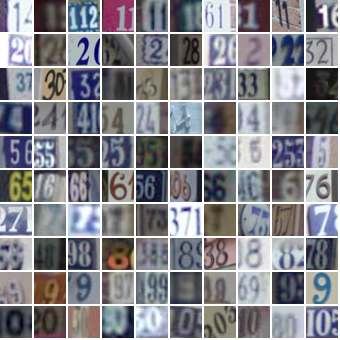
\includegraphics[width=\linewidth]{src/figures/shvn_color.png}
    \caption{Ejemplo de imagenes del conjunto de datos SHVN \cite{shvn_color}}
    \label{fig:shvn_color}
\end{figure}

\subsection{Preprocesamiento de los datos}
Para el preprocesamiento de los datos, se realizó una conversion a escala de grises de las imágenes y se normalizaron los datos,
esto se hizo por medio de la librearía OpenCV en Python con el siguiente código que se encuentra dentro de la anterior función
para el cargue de datos. 

\begin{lstlisting}
    np.array([cv2.cvtColor(img, cv2.COLOR_RGB2GRAY) / 255.0 for img in images])
\end{lstlisting}

este código permite hacer una matriz con la cantidad de imagenes y en esa matriz se agregan los datos pasados a escala de grises con
la función \textbf{\texttt{cvtColor}} especificando la imagen y el formato nuevo de color en los parametros, por último, se usa 
la division entre 255 para cada imagen y así normalizarla.

\newpage

\begin{figure}[H]
    \centering
    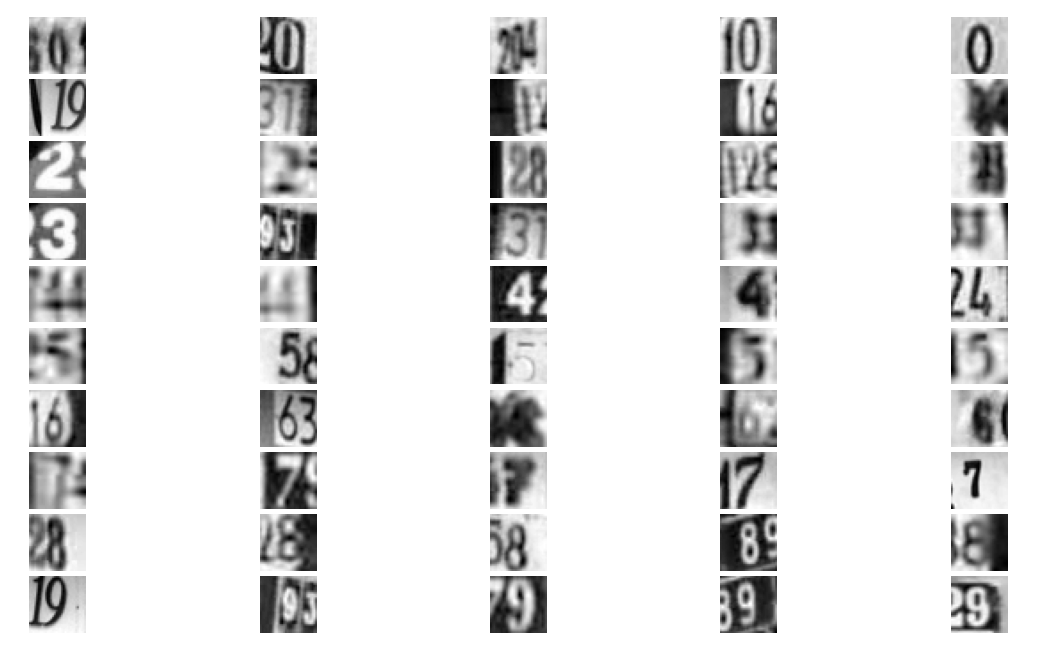
\includegraphics[width=\linewidth]{src/figures/shvn_gray.png}
    \caption{Ejemplo de imagenes del conjunto de datos SHVN en escala de grises}
    \label{fig:shvn_gray}
\end{figure}

\subsection{Implementación de la red LeNet-5}

Una vez se ha realizado el tratamiento de las imágenes se debe inicializar la red LeNet, para la construcción de esta, se usaron
las funcionalidades de \textbf{Keras} que se encuentran en la librearía de \textbf{TensorFlow}. 

Para implementar la arquitectura en código python se requiere de las siguientes lineas de código:

\begin{lstlisting}
    # Definir la arquitectura de LeNet-5
    model = models.Sequential()
    model.add(keras.Input(shape=(32, 32, 1)))
    model.add(layers.Conv2D(6, (5, 5), activation='relu'))
    model.add(layers.AveragePooling2D(pool_size=(2, 2)))
    model.add(layers.Conv2D(16, (5, 5), activation='relu'))
    model.add(layers.AveragePooling2D(pool_size=(2, 2)))
    model.add(layers.Flatten())
    model.add(layers.Dense(120, activation='relu'))
    model.add(layers.Dense(84, activation='relu'))
    model.add(layers.Dense(10, activation='softmax'))
    # Compilar el modelo
    model.compile(optimizer='adam', loss='categorical_crossentropy', metrics=['accuracy'])
\end{lstlisting}

Aquí hay varias funciones clave:

\begin{itemize}
    \item \textbf{\texttt{models.Sequential()}}: Crea una instancia del modelo secuencial de Keras. 
    Un modelo secuencial es una pila de capas donde la salida de una capa se convierte en la entrada de la siguiente capa.  
    \item \textbf{\texttt{add(layer):}} Agrega una capa al modelo.
    \item \textbf{\texttt{keras.Input(shape=(32, 32, 1))}}: Define la forma de entrada de la red. 
    La capa de entrada especifica la forma de los datos de entrada que alimentarán al modelo. 
    En este caso, los datos de entrada tienen una forma de (32, 32, 1), lo que significa que cada imagen 
    tiene una dimensión de 32x32 píxeles y un solo canal (escala de grises).
    \item \textbf{\texttt{layers.Conv2D(6, (5, 5), activation='relu')}}: Agrega una capa convolucional 2D al modelo.
    La capa de convolución aplicará 6 filtros de 5x5 píxeles a las imágenes de entrada. 
    Cada filtro aprenderá a detectar características particulares de las imágenes. 
    La función de activación utilizada es ReLU (Rectified Linear Unit), que ayuda a introducir no linealidad en el modelo.
    \item \textbf{\texttt{layers.AveragePooling2D(pool\_size=(2, 2))}}: Agrega una capa de agrupación promedio 2D al modelo.
    \item \textbf{\texttt{layers.Conv2D(16, (5, 5), activation='relu')}}: Agrega otra capa convolucional 2D al modelo.
    Esta capa aplicará 16 filtros de 5x5 píxeles a las imágenes de entrada.
    \item \textbf{\texttt{layers.Flatten()}}: Agrega una capa de aplanado al modelo.
    \item \textbf{\texttt{layers.Dense(120, activation='relu')}}: Agrega una capa densa al modelo que cuenta con 120 neuronas
    y utiliza la función de activación ReLU.
    \item \textbf{\texttt{layers.Dense(84, activation='relu')}}: Agrega otra capa densa al modelo que cuenta con 84 neuronas
    y utiliza la función de activación ReLU.
    \item \textbf{\texttt{layers.Dense(10, activation='softmax')}}: Agrega la capa de salida al modelo, que cuenta con 10 neuronas
    donde cada neurona representa un dígito del 0 al 9. La función de activación utilizada es Softmax, que convierte las salidas
    de las neuronas en probabilidades.
    \item \textbf{\texttt{model.compile(optimizer='adam', loss='categorical\_crossentropy', metrics=['accuracy'])}}:
    Esta función compila el modelo. Se especifica el optimizador Adam el cual es un algoritmo de optimización que se utiliza
    para ajustar los pesos de la red durante el entrenamiento y que se encarga de minimizar la función de pérdida. 
    La función de pérdida utilizada es la entropía cruzada categórica, que se utiliza para problemas de clasificación 
    con más de dos clases en donde su representación de salida es de tipo one-hot, por ejemplo, [0, 1, 0, 0, 0, 0, 0, 0, 0, 0].
    Por último, se especifica la métrica de precisión para evaluar el rendimiento del modelo.
\end{itemize}

Cabe aclarar que aunque estas no sean las funciones que se usaron en la implementación de la red LeNet-5, estas funciones son las
que actualente tienen un mejor rendimiento en la implementación de redes neuronales convolucionales, sin embargo, la red fue 
probada tanto con las funciones en la implementación original de la red LeNet-5 como con las funciones actuales y se realizó una
comparación de los resultados obtenidos.

\subsection{Entrenamiento de la red}

Para el entrenamiento de la red se usaron los datos de entrenamiento y se ajustaron los hiperparámetros de la red, 
uno de los parámetros importantes para el entrenamiento es la condición de parada, en este caso, se uso la precisión
del modelo de prueba para detener el entrenamiento, esto se logra con la función \textbf{\texttt{EarlyStopping}} de Keras 
y se muestra su implementación en el siguiente código:

\begin{lstlisting}
    early_stopping = EarlyStopping(
        monitor='val_accuracy',   
        patience=3,               
        min_delta=0.001,          
        mode='max',               
        verbose=1                
    )
\end{lstlisting}

En este código, se especifica que la métrica a monitorear es la precisión en los datos de validación,
se establece un umbral mínimo de mejora entre épocas de 0.001 y se especifica que se busca maximizar la precisión,
además, se establece un límite de paciencia de 3 épocas, lo que significa que si la precisión no mejora después de 3 épocas,
el entrenamiento se detendrá.

Continuando con el entrenamiento, se usó la función \textbf{\texttt{fit}} de Keras para entrenar el modelo,
a continuación se muestra el código de entrenamiento:

\begin{lstlisting}
    model.fit(
        train_images, 
        train_labels, 
        epochs=1000, 
        batch_size=128, 
        validation_data=(test_images, test_labels), 
        callbacks=[early_stopping]
        )
\end{lstlisting}

En este código, se especifican los datos de entrenamiento y las etiquetas de entrenamiento, el número de épocas de entrenamiento,
el tamaño del lote a 128, el lote es la cantidad de datos que se usan para calcular el gradiente y actualizar los pesos de la red,
es decir, se actualizan los pesos después de procesar un lote de datos y no para cada patrón. 
También se especifican los datos de validación y las etiquetas de validación, las cuales servirán para evaluar el rendimiento del modelo
durante el entrenamiento y la condición de parada. 
Por último, se especifica la función de parada temprana que se usará durante el entrenamiento.

\subsection{Evaluación de la red}

Una vez que el modelo esta entrenado simplemente se usa la función \textbf{\texttt{evaluate}} de Keras para evaluar el rendimiento
del modelo en los datos de prueba, a continuación se muestra el código de evaluación:

\begin{lstlisting}
    # Evaluar el modelo
    test_loss, test_accuracy = model.evaluate(test_images, test_labels)
    
    model_path = get_resource_path('Data/lenet_5_model.keras')
    model.save(model_path)
\end{lstlisting}

En este código, se especifican los datos de prueba y las etiquetas de prueba, y se almacenan en las variables \textbf{\texttt{test\_loss}}
y \textbf{\texttt{test\_accuracy}} respectivamente. 
La función \textbf{\texttt{evaluate}} devuelve la pérdida y la precisión del modelo en los datos de prueba, y al final se guarda el modelo
en un archivo con extensión .keras para su posterior uso sin necesidad de volver a entrenar la red.
    
La implementación de los codigos fue basada en los tutoriales de las paginas \cite{d2l} y \cite{lenet_neha}.